%% ----------------------------------------------------------------
%% Thesis.tex -- MAIN FILE (the one that you compile with LaTeX)
%% ---------------------------------------------------------------- 

% Set up the document
\documentclass[a4paper, 11pt, oneside]{Thesis}  % Use the "Thesis" style, based on the ECS Thesis style by Steve Gunn
\graphicspath{Figures/}  % Location of the graphics files (set up for graphics to be in PDF format)

% Include any extra LaTeX packages required
\usepackage[square, numbers, comma, sort&compress]{natbib}  % Use the "Natbib" style for the references in the Bibliography
\usepackage{verbatim}  % Needed for the "comment" environment to make LaTeX comments
\usepackage{vector}  % Allows "\bvec{}" and "\buvec{}" for "blackboard" style bold vectors in maths

\usepackage{tikz} % To create graphics
\usetikzlibrary{positioning}  % And this library for I really don;t know
\hypersetup{urlcolor=blue, colorlinks=true}  % Colours hyperlinks in blue, but this can be distracting if there are many links.

%% ----------------------------------------------------------------
\begin{document}
\frontmatter      % Begin Roman style (i, ii, iii, iv...) page numbering

% Set up the Title Page
\title  {Using Deep Learning techniques to improve traditional models in automatic speech recognizer on Spanish language }
\authors  {\texorpdfstring
            {\href{ma0@contraslash.com}{Mauricio Collazos}}
            {Mauricio Collazos}
            }
\addresses  {\groupname\\\deptname\\\univname}  % Do not change this here, instead these must be set in the "Thesis.cls" file, please look through it instead
\date       {\today}
\subject    {}
\keywords   {}

\maketitle
%% ----------------------------------------------------------------

\setstretch{1.3}  % It is better to have smaller font and larger line spacing than the other way round

% Define the page headers using the FancyHdr package and set up for one-sided printing
\fancyhead{}  % Clears all page headers and footers
\rhead{\thepage}  % Sets the right side header to show the page number
\lhead{}  % Clears the left side page header

\pagestyle{fancy}  % Finally, use the "fancy" page style to implement the FancyHdr headers

%% ----------------------------------------------------------------
% Declaration Page required for the Thesis, your institution may give you a different text to place here
\Declaration{

\addtocontents{toc}{\vspace{1em}}  % Add a gap in the Contents, for aesthetics

I, Mauricio Collazos, declare that this thesis titled, Using Deep Learning techniques to improve traditional models in automatic speech recognizer on Spanish language  and the work presented in it are my own. I confirm that:

\begin{itemize} 
\item[\tiny{$\blacksquare$}] This work was done wholly or mainly while in candidature for a research degree at this University.
 
\item[\tiny{$\blacksquare$}] Where any part of this thesis has previously been submitted for a degree or any other qualification at this University or any other institution, this has been clearly stated.
 
\item[\tiny{$\blacksquare$}] Where I have consulted the published work of others, this is always clearly attributed.
 
\item[\tiny{$\blacksquare$}] Where I have quoted from the work of others, the source is always given. With the exception of such quotations, this thesis is entirely my own work.
 
\item[\tiny{$\blacksquare$}] I have acknowledged all main sources of help.
 
\item[\tiny{$\blacksquare$}] Where the thesis is based on work done by myself jointly with others, I have made clear exactly what was done by others and what I have contributed myself.
\\
\end{itemize}
 
 
Signed:\\
\rule[1em]{25em}{0.5pt}  % This prints a line for the signature
 
Date:\\
\rule[1em]{25em}{0.5pt}  % This prints a line to write the date
}
\clearpage  % Declaration ended, now start a new page

%% ----------------------------------------------------------------
% The "Funny Quote Page"
\pagestyle{empty}  % No headers or footers for the following pages

\null\vfill
% Now comes the "Funny Quote", written in italics
\textit{This is the only funny part of this document, and this does not is even funny}

\begin{flushright}
Mauricio Collazos
\end{flushright}

\vfill\vfill\vfill\vfill\vfill\vfill\null
\clearpage  % Funny Quote page ended, start a new page
%% ----------------------------------------------------------------

% The Abstract Page
\addtotoc{Abstract}  % Add the "Abstract" page entry to the Contents
\abstract{
\addtocontents{toc}{\vspace{1em}}  % Add a gap in the Contents, for aesthetics

In the last decade all majors fields in Artificial Intelligence (AI) has been affected by Deep Learning (DL) techniques due significant improvements on Image Processing \cite{KrizhevskyImageNetNetworks}, Automatic Speech Recognition (ASR) also has been affected \cite{XuedongHuangAlexAceroHsiao-WuenHon201,HwangSubphoneticRecognition}.

In this thesis we walk through traditional techniques in ASR and use DL to improve results

}

\clearpage  % Abstract ended, start a new page
%% ----------------------------------------------------------------

\setstretch{1.3}  % Reset the line-spacing to 1.3 for body text (if it has changed)

% The Acknowledgements page, for thanking everyone
\acknowledgements{
\addtocontents{toc}{\vspace{1em}}  % Add a gap in the Contents, for aesthetics

First of all I thank God for the opportunities.

To my lovely family, Nancy, Blanca and Angie

And everyone else involved in this major step of my life

Almost forgot my despicable thesis advisor \ldots Just kidding, this would not even been possible without Raul.


}
\clearpage  % End of the Acknowledgements
%% ----------------------------------------------------------------

\pagestyle{fancy}  %The page style headers have been "empty" all this time, now use the "fancy" headers as defined before to bring them back


%% ----------------------------------------------------------------
\lhead{\emph{Contents}}  % Set the left side page header to "Contents"
\tableofcontents  % Write out the Table of Contents

%% ----------------------------------------------------------------
\lhead{\emph{List of Figures}}  % Set the left side page header to "List if Figures"
\listoffigures  % Write out the List of Figures

%% ----------------------------------------------------------------
\lhead{\emph{List of Tables}}  % Set the left side page header to "List of Tables"
\listoftables  % Write out the List of Tables

%% ----------------------------------------------------------------
\setstretch{1.5}  % Set the line spacing to 1.5, this makes the following tables easier to read
\clearpage  % Start a new page
\lhead{\emph{Abbreviations}}  % Set the left side page header to "Abbreviations"
\listofsymbols{ll}  % Include a list of Abbreviations (a table of two columns)
{
% \textbf{Acronym} & \textbf{W}hat (it) \textbf{S}tands \textbf{F}or \\
\textbf{ASR} & \textbf{A}utomatic \textbf{S}peech \textbf{R}ecognition \\
\textbf{DL} & \textbf{D}eep \textbf{L}earning

}

%% ----------------------------------------------------------------
% \clearpage  % Start a new page
% \lhead{\emph{Physical Constants}}  % Set the left side page header to "Physical Constants"
% \listofconstants{lrcl}  % Include a list of Physical Constants (a four column table)
% {
% Constant Name & Symbol & = & Constant Value (with units) \\
% Speed of Light & $c$ & $=$ & $2.997\ 924\ 58\times10^{8}\ \mbox{ms}^{-\mbox{s}}$ (exact)\\

% }

%% ----------------------------------------------------------------
% \clearpage  %Start a new page
% \lhead{\emph{Symbols}}  % Set the left side page header to "Symbols"
% \listofnomenclature{lll}  % Include a list of Symbols (a three column table)
% {
% % symbol & name & unit \\
% $a$ & distance & m \\
% $P$ & power & W (Js$^{-1}$) \\
% & & \\ % Gap to separate the Roman symbols from the Greek
% $\omega$ & angular frequency & rads$^{-1}$ \\
% }
%% ----------------------------------------------------------------
% End of the pre-able, contents and lists of things
% Begin the Dedication page

\setstretch{1.3}  % Return the line spacing back to 1.3

\pagestyle{empty}  % Page style needs to be empty for this page
\dedicatory{For my and all my friends\ldots}

\addtocontents{toc}{\vspace{2em}}  % Add a gap in the Contents, for aesthetics


%% ----------------------------------------------------------------
\mainmatter	  % Begin normal, numeric (1,2,3...) page numbering
\pagestyle{fancy}  % Return the page headers back to the "fancy" style

% Include the chapters of the thesis, as separate files
% Just uncomment the lines as you write the chapters

\chapter{Project Proposal}

In this first chapter we describe the main goal of this project, including the problem definition, justification, objectives, methodology and expected results.
\section{Problem definition}

Automatic Speech Recognition (ASR) has been one of the most investigated topic in Speech Processing \cite{Rabiner1993FundamentalsRecognition}. Many difficulties and open questions still remain unsolved, problems related to increasing dictionary size (more than 50.000 words), robust speech recognition (capability of recognition on noisy environments), speaker independence (capability for understand any speaker), spontaneous speech phenomena (false starts, out of vocabulary words, mumbling), distant speech recognition (the speaker is located far from the input source) and so on \cite{Trentin2001ARecognition}.

Although all this work, precision on ASR task related in Spanish Language does not exceed 70 percent of accuracy. Open Source resource are not enough to train robust models used in literature.

With this work we aim to minimize the gap between long studies languages like English and Spanish, providing effective implementations of frameworks, algorithms, models, techniques and methodologies to Spanish merging traditional frameworks with DL optimization.

The results are restricted to existing open corpus in Spanish Language and two proposal of new corpus: Open Speech Corpus \cite{QUOTE REQUIRED} and Libri Speech Spanish \cite{QOUTE REQUIRED}

\section{Justification}

ASR is a major field of research. Leader technology companies are leading investigation on modern systems building Intelligent Personal Assistants, as the case of Google with Google Home\cite{Li2017}, Microsoft with Cortana\cite{Xiong2017}, Apple with Siri and Amazon with Echo.

Applications of ASR technologies are broad and useful for numerous fields, including marketing, technical support, finances, personal assistants, monitoring, and more.

Speech represents a natural interface of communication for humans. Some psychologist consider that language is the key of human knowledge \cite{QOUTE REQUIRED} and speech still maintain as a key way to pass and store information.

\section{Objectives}

We present general and specific objectives in this section

\subsection{General objective}

Adapt Deep Learning relevant frameworks, algorithms, models, techniques and methodologies to improve Automatic Speech Recognition on Spanish Language.

\subsection{Specific objectives}

\begin{itemize}
    \item Select relevant algorithms, models, techniques and methodologies to improve ASR
    \item Collect Spanish resources to develop improvements on ASR
    \item Implement solutions based on DL to improve ASR precision
    \item Measure improvements of implementations achieved
\end{itemize}

\section{Methodology}

To accomplish each specific objectives the methodology  to be used start with a literature exploration of academic publications using hybrid techniques on ASR combining traditional frameworks and DL implementations. Then select most relevant resources to implement.

Simultaneously select open data to work in Spanish, including existing annotated corpus and adapting non-annotated corpus to work with tools selected.

With tools selected, implement required functionality and adapt to work in Spanish.

Finally, measure traditional techniques performance, response time, training time and resources required comparing to implementation proposed.

\section{Expected results}

With this thesis we expect two visible results:

\begin{itemize}
    \item An open framework to build ASR systems using DL and
    \item a larger corpus to work with ASR in Spanish
\end{itemize}




 % Introduction

\chapter{State of the art}
\section{Introduction}
Automatic Speech Recognition (ASR) has been one of the most investigated topic in Speech Processing \cite{Rabiner1993FundamentalsRecognition}. Many difficulties and open questions still remain unsolved, problems related to increasing dictionary size (more than 50.000 words), robust speech recognition (capability of recognition on noisy environments), speaker independence (capability for understand any speaker), spontaneous speech phenomena (false starts, out of vocabulary words, mumbling), distant speech recognition (the speaker is located far from the input source) and so on \cite{Trentin2001ARecognition}.


Traditional architectures of an ASR are composed by 4 elements as illustrated on Fig. 1: a Signal Processing and Feature Extraction (FE), an Acoustic Model (AM) a Language Model (LM) and a Hypothesis Search.

\begin{figure}
\centering
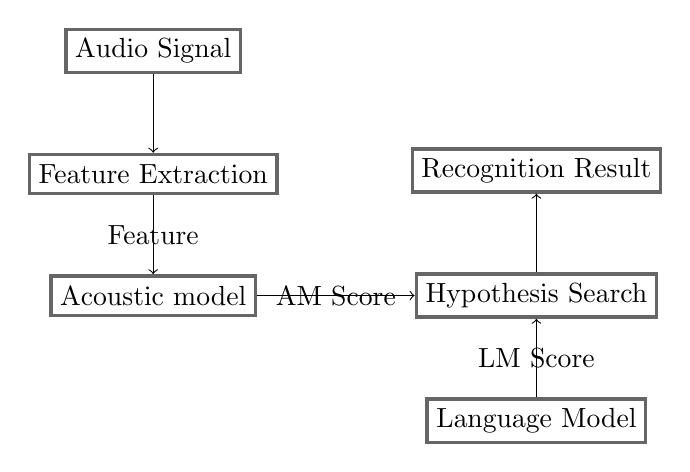
\begin{tikzpicture}[
squarednode/.style={rectangle, draw=black!60, fill=white!5, very thick, minimum size=5mm},
]
%Nodes
\node[squarednode]      (am)                              {Acoustic model};
\node[squarednode]        (fe)       [above=of am] {Feature Extraction};
\node[squarednode]        (wave)       [above=of fe] {Audio Signal};
\node[squarednode]      (hypothesis)       [right=2cm of am] {Hypothesis Search};
\node[squarednode]        (lm)       [below=of hypothesis] {Language Model};
\node[squarednode]        (result)       [above=of hypothesis] {Recognition Result};
 
%Lines
\draw[->] (wave.south) -- (fe.north);
\draw[->] (fe.south) -- node{Feature}(am.north);
\draw[->] (am.east) -- node{AM Score}(hypothesis.west);
\draw[->] (lm.north) -- node{LM Score}(hypothesis.south);
\draw[->] (hypothesis.north) -- (result.south);
\end{tikzpicture}

\caption{Classic architecture \cite{YuAutomaticApproach}}
\label{fig:fig1}
\end{figure}

The Feature Extraction (FE) process is usually called Front End because is the first step of Speech Recognition, its labor is to enhance the speech, removing distortions noise and transforming the wave in a representation that can be used from the AM, usually this transformation is made using Mel Frequency Cepstral Coefficients (MFCC) \cite{Davis1980ComparisonSentences}, Spectral Transform-Perceptual Linear Prediction (RASTA-PLP) \cite{Hermansky1990PerceptualSpeech}, log-RASTA-PLP that is used to modulate the spectrogram and improve performance on reverberant environments \cite{Kingsbury1998RobustSpectrogram} or the Model of Auditory Perception\cite{Dau1996AStructure.} (also abbreviated PEMO \cite{Kleinschmidt2001CombiningRecognition}) that aims to simulate the auditory system. 

The Acoustic Model (AM) estimates the probability for the transformed audio input given a known context and returns a score for the variable-length. This process is usually made with an HMM \cite{RabinerARecognition} in combination with Gaussian Mixture Models (GMM), Support Vector Machines, Conditional Random Fields and Artificial Neural Networks \cite{Jurafsky2000SpeechRecognition}. Nowadays, techniques based on DNN has gained feasibility and approaches like Context Dependent Deep Neural Networks Hidden Markov Models (CD-DNN-HMM) are used instead \cite{Deng2012}. 

The Language Model (LM) estimates the probability of a hypothesized word sequence; this approach uses N-grams with a very large collection of text. Usually specific corpora are used to improve classification on closed domains, but new approximations try to exploit the size of the web to build dynamic Language Models\cite{Oger2014Web-basedRecognition}.

Finally the Hypothesis Search merges the output of the AM and the LM. 

In this paper we describe a brief history of ASR. In section 2 we cover the beginnings on the early 50's until new industry products like Google Home and Amazon Echo. We define the classification of ASR in section 3 covering aspects like speech mode, speaker mode and vocabulary size. Section 4 describes recent work on topics like Robust Speech Recognition, Spoken Language Understanding (SLU), Distant Speech Recognition,  single channel multi-speaker recognition, and Deep Neural Networks approaches. In the last section we describe corpora to work in English and Spanish and propose a new corpus for Large Vocabulary Speaker Independent Robust Speech Recognition Systems.

\section{History}
First approaches to ASR system were made on Bell Labs on 50's, where K.H. Davis, R. Biddulph and S. Balashek construct a circuit that recognize digits from a single speaker with 97\% accuracy \cite{Davis1952AutomaticDigits}. Then H. F. Olson extend this approach to build a Phonetic Typewriter \cite{Olson1957PhoneticTypewriter}. Both approaches relies on spectral resonances measuring with an analog filter bank. In 1959 at University College London, D. Fry and P. Denes extend the merely acoustic approach adding statistic information about frequencies of phonemes in English \cite{BritishInstitutionofRadioEngineers.1959TheEngineers.}. 


In the 60's Japaneses companies worked on a hardware approach, using different channels to filter vowels on their own pitches \cite{Sakai1961TheMechanism,Nagata1964SpokenLanguage}. Simultaneously RCA Labs worked on a set of time normalization methods to identify starts and ends of speech\cite{Martin1964SPEECHTECHNIQUES.}, while T. Vintsiuk develop a set of dynamic programming methods that fits speech recognition problems \cite{Vintsyuk1972SpeechProgramming} These both advances marked the next 20 years of research, allowing different companies all over the world to achieve isolated word recognition \cite{Velichko1970AutomaticWords,Sakoe1978DynamicRecognition,Itakura1975MinimumRecognition}.

After the break of recognize isolated words in 70's the next big challenge for researches was continuous speech recognition so the statistical approaches based on Hidden Markov Models (HMM) gain importance \cite{RabinerARecognition}. At the same time, techniques based on Artificial Neural Networks (ANN) where implemented \cite{Waibel1989PhonemeNetworks}  but the popularity of HMM and the computing capacity did not allow this technique to work in this decade.

The end of the 80's and the beginning of the 90's was full of systems that focuses on Continuous Speech Recognition, standing out SPHINX by Carnegie Mellon University (CMU) \cite{Lee1990AnSystem}, BYBLOS \cite{ChowBYBLOS:System}, the Lincoln Robust Speech Recognizer \cite{PaulTheRecognizer} and the MIT Summit Speech Recognition System \cite{Zue1989TheReport}. Many of these systems use a HMM approach mixed with a Gaussian Mixture Models using Senones: a sub-phonetic unit which allow each phone sub model to share and cluster its state\cite{HwangSubphoneticRecognition}.

The new millennium begun with new problems: noise and larger vocabulary. Those problems force the technology to adapt the Continuous Speech Recognition into a Robust Continuous Speech Recognition \cite{SieglerOnSystems,MirghaforiTowardsASR}.  To reduce noise one approach was to reduce bandwidth of the sound perception and create a modulation spectrogram to reduce reverberation and noise perception \cite{Kingsbury1998RobustSpectrogram}. Also segment the audio wave and identify unreliable segments using marginalization and state-based data imputation combined with energy bounds which improved performance on noisy channels. \cite{Cooke2001RobustData}. For large vocabulary problems new hybrid approaches begun for improve performance combining existing HMM with ANN on vowel recognition \cite{BourlardABands}. Also by extending the features with Articulatory and pseudo Articulatory parameters they helped to improve both large vocabulary and noise \cite{Kirchhoff2002CombiningRecognition}

A big milestone was achieved in 2008 when Artificial Intelligence (AI) met Graphical Processing Units (GPU) for image classification \cite{KrizhevskyImageNetNetworks}; this approach unleash a whole new perspective using ANN with large hidden layers, creating a new concept: Deep Neural Networks (DNN).  The ASR main approach until these date was using HMM and Gaussian Mixture Models (GMM) \cite{XuedongHuangAlexAceroHsiao-WuenHon201,HwangSubphoneticRecognition}, now first approach became to create a hybrid models based on these research and the deep concepts. One of the first approach was made with researchers at Microsoft, creating the first Context Dependent Deep Neural Network Hidden Markov Model (CD-DNN-HMM) and showing an improvement of almost three points using just 5 hidden layers \cite{Xiong2017}. 

ASR continues as a major field of research. Leader technology companies are leading investigation on modern systems building Intelligent Personal Assistants, as the case of Google with Google Home\cite{Li2017}, Microsoft with Cortana\cite{Xiong2017}, Apple with Siri and Amazon with Echo.

\section{ASR Classification}
Speech Processing is a wide subproblem in Natural Language Processing (NLP) and includes Recognition, Analysis/Synthesis and Coding/Production. Speech Recognition problem is also divided in Automatic Speech Recognition, Speaker Recognition and Language Identification.

ASR can be classified by its Mode of Speech, the Speaker or the Vocabulary Size, each classification has its own subclassifications and are described next:
\subsection{Speech Mode}
\subsubsection{Isolated Speech}
Isolated word recognizers identify words separated by a time window of silence. These systems have "Listen/Not-Listen" states, where the speaker must wait between words.
\subsubsection{Continuous Speech}
Continuous Speech Recognizer allow users to speak naturally, and the system split the words determining word boundaries.
\subsection{Speaker Mode}
\subsubsection{Speaker Dependent}
Speaker Dependent systems recognize audio samples from a predefined set of speakers.
These systems learn the unique individual characteristics of a single person voice. A new user must first train the system by a voice configuration protocol.
\subsubsection{Speaker Independent}
Speaker Independent Systems recognize audio samples from any speaker, in contrast to Speaker Dependent systems, these system are less accurate and try to avoid this problem defining a closed domain.
\subsubsection{Speaker Adaptive}
Speaker Adaptive systems sit between Speaker Dependent and Speaker Independent systems, these system aims to define a normalization method to parametrize speakers. i-Vectors is a technique that simplify the process \cite{Xiong2017}, and also prove to work with DNN architectures  \cite{MiaoIEEE/ACMI-vectors}
\subsection{Vocabulary Size}
Although it does not exist a formal definition of vocabulary size, most researches agrees on quantity notation on definitions based on power of tens: \textbf{Small Vocabulary} consists of tens of words, a \textbf{Medium vocabulary} consists of hundreds of words, a \textbf{Large vocabulary} consists of thousands of words and a \textbf{Very Large Vocabulary} consists of tens thousands of words.
\section{Hot topics in ASR}

Last decade has been a great time for Artificial Intelligence, significant milestones have been achieved and new research questions has been opened. We present popular topics in ASR research in Table 1 and explain briefly every hot topic in each subsection.

\subsection{Robust Speech Recognition}
Robust Speech Recognition is a term designed to ASR systems that can perform recognition with low fidelity audio input, including noisy environments, distance from input source, false starts, unknown words and mumbling. The need of a robust ASR begun at mid 90's where the experimental results did not work in real scenarios because the distortion of the input wave. Reduce noise with filters does not work with high-noise conditions \cite{Barker2005DecodingSources}. Front-End ASR have the task to clean the input wave and extract relevant features to be processed by the Back-End ASR. Ghanbari and Reza use a new concept based on Wavelet Transform instead the traditional Fourier Transform giving a new architecture to work and shows to improve performance in environments with white, pink and multi-talker noises\cite{Ghanbari2006APackets}. Cooke and Green propose to classify a priori unreliable segments of speech and then work in the final hypothesis with the missing information first using marginalization and also state-based data imputation. With marginalization the results improve the hypothesis but using just state-based data imputation the front end can filter data in a way that can be processed with regular decoders\cite{Cooke2001RobustData}.  Other approaches does not assume just noisy environments but heterogeneous environments. Instead of filter noise, processors aims to separate the sources\cite{Barker2005DecodingSources}, later this technique was improved to have single channel multi-speaker speech recognition\cite{Rennie2010Single-ChannelRecognition}.
\subsection{Spoken Language Understanding}
Natural Language Understanding (NLU) is another field of investigation of Natural Language Processing. ASR systems outputs the best hypothesis and these output became the input of other systems that extract information and reply to the users. Hakkani and Bechet propose to use Word Confusion Networks (WCN) to improve Named Entity Recognition (NER) \cite{Hakkani-Tur2006BeyondUnderstanding}. Spoken Language have more features to extract than Written Language, and prosodic features can outperform the results of a regular NLU system adding multiple hypothesis to the process queue\cite{DeMori2008SpokenUnderstanding}. Knowledge Representation and Semantic Confidence merge in the ASR stack combining task related to NLU, requiring more features annotated on the training corpora \cite{Baker2009DevelopmentsEducation} and the adaptations of models, algorithms and search \cite{Baker2009UpdatedEducation} but merging ASR with NLU will be the foundation of AI in a near future.
\subsection{Distant Speech Recognition}
ASR systems are the entrance door for Spoken Dialogue Systems, a subsection of Human Computer Interaction (HCI). Humans can't have a microphone attached to their body at any time so a system can listen, fixed position microphones with humans moving around speaking, and this problem becomes with new challenges for ASR, like additive noise and reverberation \cite{Woelfel2009DistantRecognition}. Reverberation is a wide open research problem and multiple approaches are implemented to achieve a clean audio output \cite{Tsilfidis2013AutomaticPreprocessing,Ma2013TheChallenge,Vacher2015OnAutomation}
\subsection{Single Channel multi-speaker Recognition}
Single Microphone can often record data from multiple speakers. Speaker segmentation are needed for  improve ASR with single speaker information. Techniques with DNN have shown important advances in this topics building a full architecture with Weighted  Finite State Transducers \cite{Weng2015DeepRecognition} and Data driven approximations \cite{Du2016ANetworks}
\subsection{Deep Neural Networks}
Using Artificial Neural Networks to improve Back-End architectures are a studied field\cite{Trentin2001ARecognition}. With Deep Learning, ANN with several layers come as a powerful approach to improve decoders. Context Dependent DNN-HMM are a solid approach to migrate existing HMM-GMM systems\cite{Deng2012}. Full frameworks has been built on industry to achieve high level ASR systems\cite{Zou2014Mariana:Applications}. Adaptive approaches try to reduce reverberation and noise in a Front-End\cite{Narayanan2014ImprovingTraining}. Deep Learning techniques are sitting on every level of ASR systems trying to improve performance
\begin{landscape}
\begin{table}
\centering
\caption{Hot topics on ASR}
\label{tab1}
\begin{tabular}{|l|l|}
\hline
% Begin of the mulitiple line
\multirow{8}{*}{Robust Speech Recognition}  
% Row1l
& \multicolumn{1}{l}{Reconstruction of missing features for robust speech recognition \cite{Raj2004ReconstructionRecognition}} \\ \cline{2-2} 
% Row
& \multicolumn{1}{l}{Decoding speech in the presence of other sources\cite{Barker2005DecodingSources}}  \\ \cline{2-2} 
% Row
& \multicolumn{1}{l}{A new approach for speech enhancement based on the adaptive thresholding of the wavelet packets\cite{Ghanbari2006APackets}} \\ \cline{2-2}
% Row
& \multicolumn{1}{l}{Signal Subspace Speech Enhancement and Its Application to Noise Robust Speech Recognition\cite{Hermus2006ARecognition}} \\\cline{2-2}
% Row
& \multicolumn{1}{l}{A study on integrating acoustic-phonetic information into lattice rescoring for automatic speech recognition \cite{Siniscalchi2009ARecognition}} \\\cline{2-2}
% Row
& \multicolumn{1}{l}{Discriminative feature extraction for speech recognition using continuous output codes \cite{Dehzangi2012DiscriminativeCodes}} \\\cline{2-2}
% Row
& \multicolumn{1}{l}{A new framework for robust speech recognition in complex channel environments \cite{He2014AEnvironments}} \\\cline{2-2}
% Row
& \multicolumn{1}{l}{Automatic Complexity Control of Generalized Variable Parameter HMMs for Noise Robust Speech Recognition \cite{Su2014AutomaticRecognition}} \\\hline


% End Row
% Begin of the multiple line
\multirow{4}{*}{Spoken Language Understanding}  
% Row
& \multicolumn{1}{l}{Using word confusion networks in spoken language understanding\cite{Hakkani-Tur2006BeyondUnderstanding}} \\\cline{2-2}
% Row
& \multicolumn{1}{l}{Spoken Language Understanding \cite{DeMori2008SpokenUnderstanding}}  \\\cline{2-2}
% Row
& \multicolumn{1}{l}{Developments and directions in speech recognition and understanding \cite{Baker2009DevelopmentsEducation,Baker2009UpdatedEducation}} \\\cline{2-2}
% Row
& \multicolumn{1}{l}{Spoken language understanding\cite{Ye-YiWang2005SpokenUnderstanding}} \\\hline
% End Row
% Begin of the multiple line
\multirow{4}{*}{Distant Speech Recognition}  
% Row
& \multicolumn{1}{l}{Automatic speech recognition performance in different room acoustic environments with and without dereverberation preprocessing \cite{Tsilfidis2013AutomaticPreprocessing}} \\\cline{2-2}
% Row
& \multicolumn{1}{l}{The PASCAL CHiME speech separation and recognition challenge \cite{Ma2013TheChallenge}}  \\\cline{2-2}
% Row
& \multicolumn{1}{l}{On Distant Speech Recognition for Home Automation \cite{Vacher2015OnAutomation}} \\\cline{2-2}
% Row
& \multicolumn{1}{l}{Strategies for distant speech recognitionin reverberant environments \cite{Delcroix2015StrategiesEnvironments}} \\\hline
% Begin of the mulitiple line
\multirow{3}{*}{Single Channel muti-speaker Recognition}  
% Row
& \multicolumn{1}{l}{Single-Channel Multitalker Speech Recognition \cite{Rennie2010Single-ChannelRecognition}} \\\cline{2-2}
% Row
& \multicolumn{1}{l}{Deep Neural Networks for Single-Channel Multi-Talker Speech Recognition \cite{Weng2015DeepRecognition}}  \\\cline{2-2}
% Row
& \multicolumn{1}{l}{A Regression Approach to Single-Channel Speech Separation Via High-Resolution Deep Neural Networks\cite{Du2016ANetworks}} \\\hline
% Row
% End Row
% Begin of the mulitiple line
\multirow{4}{*}{Deep Neural Networks}  
% Row
& \multicolumn{1}{l}{Context-Dependent Pre-trained Deep Neural Networks for Large Vocabulary Speech Recognition \cite{Deng2012}} \\\cline{2-2}
% Row
& \multicolumn{1}{l}{Environmentally robust ASR front-end for deep neural network acoustic models\cite{Yoshioka2015EnvironmentallyModels}}  \\\cline{2-2}
% Row
& \multicolumn{1}{l}{Mariana: Tencent Deep Learning Platform and its Applications \cite{Zou2014Mariana:Applications}} \\\cline{2-2}
% Row
& \multicolumn{1}{l}{Improving robustness of deep neural network acoustic models via speech separation and joint adaptive training\cite{Narayanan2014ImprovingTraining}}  \\\cline{2-2}
% Row
& \multicolumn{1}{l}{Neural Network Based Multi-Factor Aware Joint Training for Robust Speech Recognition \cite{Qian2016NeuralRecognition}} \\\cline{1-2}
% End Row

\end{tabular}
\end{table}
\end{landscape}

% \bibliographystyle{splncs04} 
\section{Corpus}
Corpus is a latin word that represent a datasets of linguistic resources and are used to train Machine Learning Algorithm algorithms. We present popular speech corpus in English and Spanish and its main features.
\subsection{Speech English Corpus }
\begin{table}
\centering
\caption{Popular English Speech Corpus}
\label{tab2}
\begin{tabular}{|l|l|}
\hline
Database & Style\\
\hline
TIMIT \cite{PriceTheRecognition} & Read  \\
\hline
DARPA Resource Management \cite{Lucke1992ExpandingCorpus} & Read  \\
\hline
Switchboard \cite{Godfrey1992SWITCHBOARD:Development} & Spontaneous \\
\hline
Cambridge Read News \cite{RobinsonWSJCAM0:RECOGNITION} & Read  \\
\hline
Call Home \cite{Fu-HuaLiuSpeechCorpus} & Spontaneous  \\
\hline
Aurora Digits \cite{EvansEfficientCorpus} & Read \\
\hline
FISHER \cite{CieriTheSpeech-to-Text} & Spontaneous \\
\hline
LIBRISPEECH \cite{PanayotovLIBRISPEECH:BOOKS} & Read \\
\hline
\end{tabular}
\end{table}

TIMIT corpus was created in 1986 and aims to identify phones based on more than 630 speakers of 8 major dialects and each sentence is considered a phonetically rich sentence. TIMIT was a standard to test ASR systems and contains 5.4 hours of speech \cite{PriceTheRecognition}.

DARPA Resource Management is a corpus designed to create continuous speech recognition systems, the corpus is divided in two parts, the first part contains resources from 160 speakers reading sentences and contains more than 25.000 utterances, part two contains audio from 12 subjects and a set of 600 sentences. \cite{Lucke1992ExpandingCorpus}

SWITCHBOARD is a corpus with over 240 hours of spontaneous conversations; contains more than 500 speakers. This corpus was created to create continuous speech recognition systems \cite{Godfrey1992SWITCHBOARD:Development}.

Cambridge Read News is a corpus recorded at Cambridge University and is derived from the Wall Street Journal Text Corpus, the database consists on 140 speakers speaking about 110 utterances\cite{RobinsonWSJCAM0:RECOGNITION}

CALL HOME is a multi language corpus initially created for translate Mandarin to Spanish but with the time more languages was added like Portuguese and Spanish. The English Corpus has 18.3 Hours \cite{Fu-HuaLiuSpeechCorpus}.

AURORA is a little corpus focused on digits it contains only 11 words, 9 digits, 0 and silence. The aim of this project was to test simple ASR systems.

FISHER corpus is a telephone based corpus, derived from DARPA EARS, contains more than 16.000 conversations and a over 2.000 hours of annotated data\cite{CieriTheSpeech-to-Text}.

LIBRISPEECH is an effort from John Hopkins University and is derived from LibroVox project, a project that collect audio books and publish it with open licenses the corpus contains over 1000 hours of audio \cite{PanayotovLIBRISPEECH:BOOKS}.
\cite{EvansEfficientCorpus}.
\subsection{Spanish Corpora}
\begin{table}
\centering
\caption{Corpus used for Speech Recognition in Spanish}
\label{tab2}
\begin{tabular}{|l|l|}
\hline
Database & Style \\
\hline
Voxforge & Read   \\
\hline
CIEMPIESS\cite{Hernandez-MenaCIEMPIESS:Corpus} & Spontaneous  \\
\hline
DIMEx100\cite{Pineda2004DIMEx100:Spanish} & Read  \\
\hline
Albayzín\cite{CampilloAlbayzinEvaluation} & Read  \\
\hline
\end{tabular}
\end{table}

VOXFORGE is a project to crowd source audio input with multiple languages. The Spanish version  has over 51 hours of audio data, however the audio inputs are limited, having only 971 words.

CIEMPIESS is a spontaneous corpus from a Radio station at Mexico, it contains 17 hours of audio recorded from a FM podcast at Mexico DF, the corpus is annotated phonetically using a simple phoneme representation and another annotation using allophones \cite{Hernandez-MenaCIEMPIESS:Corpus}.

DIMEx100 is a read corpus from 100 speaker and each one read 50 individual phrases extracted from Corpus230 \cite{Villasenor-Pineda2004ExperimentsWeb} and aims to be phonetically balanced \cite{Pineda2004DIMEx100:Spanish}.

Albayzín is a Text to Speech corpus evaluation, recorded from 304 castillian speakers and contains over 6.800 utterances and is phonetically balanced. 1000 sentences are phonetically segmented. This corpus is distributed by European Language Resource Association \cite{CampilloAlbayzinEvaluation}.

With this examples we compare Spanish resources to build ASR systems and usually data are not enough to build a Large Vocabulary Speaker Independent ASR. Researchers usually collect its own data and made experiments using a relative small vocabulary \cite{Becerra2017,Celis2017AcousticRegion}.
\section{Open Speech corpus}

Identifying limitations on data to generate Speaker Independent Large Vocabulary ASR, we propose a new corpus for Spanish called OPEN SPEECH CORPUS for Spanish to aim this goal using data gathered with a mobile phone via and Android application.

So far the proposed corpus has more than 42 hours of audio of 77 speakers based on readings of Latin American writers. The project still having new data inputs and aims to get 100 hours of annotated audio. The corpus has 22295 different words assuring variability and diversity on the phones recorded.

A second data collection is proposed using single word readings to create a seed model for use in open source tools like Aeneas, Penn Forced Aligner, Prosodylab-Aligner\cite{Gorman2011Prosodylab-aligner:Speech}, to align open open speech databases like LibriBox that has over 325 books and increase the open data to make research. % Background Theory 

%\input{Chapters/Chapter3} % Experimental Setup

%\input{Chapters/Chapter4} % Experiment 1

%\input{Chapters/Chapter5} % Experiment 2

%\input{Chapters/Chapter6} % Results and Discussion

%\input{Chapters/Chapter7} % Conclusion

%% ----------------------------------------------------------------
% Now begin the Appendices, including them as separate files

\addtocontents{toc}{\vspace{2em}} % Add a gap in the Contents, for aesthetics

\appendix % Cue to tell LaTeX that the following 'chapters' are Appendices

% \chapter{An Appendix}

Lorem ipsum dolor sit amet, consectetur adipiscing elit. Vivamus at pulvinar nisi. Phasellus hendrerit, diam placerat interdum iaculis, mauris justo cursus risus, in viverra purus eros at ligula. Ut metus justo, consequat a tristique posuere, laoreet nec nibh. Etiam et scelerisque mauris. Phasellus vel massa magna. Ut non neque id tortor pharetra bibendum vitae sit amet nisi. Duis nec quam quam, sed euismod justo. Pellentesque eu tellus vitae ante tempus malesuada. Nunc accumsan, quam in congue consequat, lectus lectus dapibus erat, id aliquet urna neque at massa. Nulla facilisi. Morbi ullamcorper eleifend posuere. Donec libero leo, faucibus nec bibendum at, mattis et urna. Proin consectetur, nunc ut imperdiet lobortis, magna neque tincidunt lectus, id iaculis nisi justo id nibh. Pellentesque vel sem in erat vulputate faucibus molestie ut lorem.

Quisque tristique urna in lorem laoreet at laoreet quam congue. Donec dolor turpis, blandit non imperdiet aliquet, blandit et felis. In lorem nisi, pretium sit amet vestibulum sed, tempus et sem. Proin non ante turpis. Nulla imperdiet fringilla convallis. Vivamus vel bibendum nisl. Pellentesque justo lectus, molestie vel luctus sed, lobortis in libero. Nulla facilisi. Aliquam erat volutpat. Suspendisse vitae nunc nunc. Sed aliquet est suscipit sapien rhoncus non adipiscing nibh consequat. Aliquam metus urna, faucibus eu vulputate non, luctus eu justo.

Donec urna leo, vulputate vitae porta eu, vehicula blandit libero. Phasellus eget massa et leo condimentum mollis. Nullam molestie, justo at pellentesque vulputate, sapien velit ornare diam, nec gravida lacus augue non diam. Integer mattis lacus id libero ultrices sit amet mollis neque molestie. Integer ut leo eget mi volutpat congue. Vivamus sodales, turpis id venenatis placerat, tellus purus adipiscing magna, eu aliquam nibh dolor id nibh. Pellentesque habitant morbi tristique senectus et netus et malesuada fames ac turpis egestas. Sed cursus convallis quam nec vehicula. Sed vulputate neque eget odio fringilla ac sodales urna feugiat.

Phasellus nisi quam, volutpat non ullamcorper eget, congue fringilla leo. Cras et erat et nibh placerat commodo id ornare est. Nulla facilisi. Aenean pulvinar scelerisque eros eget interdum. Nunc pulvinar magna ut felis varius in hendrerit dolor accumsan. Nunc pellentesque magna quis magna bibendum non laoreet erat tincidunt. Nulla facilisi.

Duis eget massa sem, gravida interdum ipsum. Nulla nunc nisl, hendrerit sit amet commodo vel, varius id tellus. Lorem ipsum dolor sit amet, consectetur adipiscing elit. Nunc ac dolor est. Suspendisse ultrices tincidunt metus eget accumsan. Nullam facilisis, justo vitae convallis sollicitudin, eros augue malesuada metus, nec sagittis diam nibh ut sapien. Duis blandit lectus vitae lorem aliquam nec euismod nisi volutpat. Vestibulum ornare dictum tortor, at faucibus justo tempor non. Nulla facilisi. Cras non massa nunc, eget euismod purus. Nunc metus ipsum, euismod a consectetur vel, hendrerit nec nunc.	% Appendix Title

%\input{Appendices/AppendixB} % Appendix Title

%\input{Appendices/AppendixC} % Appendix Title

\addtocontents{toc}{\vspace{2em}}  % Add a gap in the Contents, for aesthetics
\backmatter

%% ----------------------------------------------------------------
\label{Bibliography}
\lhead{\emph{Bibliography}}  % Change the left side page header to "Bibliography"
\bibliographystyle{unsrtnat}  % Use the "unsrtnat" BibTeX style for formatting the Bibliography
% \bibliography{Bibliography}  % The references (bibliography) information are stored in the file named "Bibliography.bib"
\bibliography{mendeley_v2.bib}

\end{document}  % The End
%% ----------------------------------------------------------------